\chapter[Sensor PCB assembly]{Sensor \pcb\ assembly}

\section[Sensor PCB version 1.2]{Sensor \pcb\ version 1.2}

\begin{figure}
  \centering
  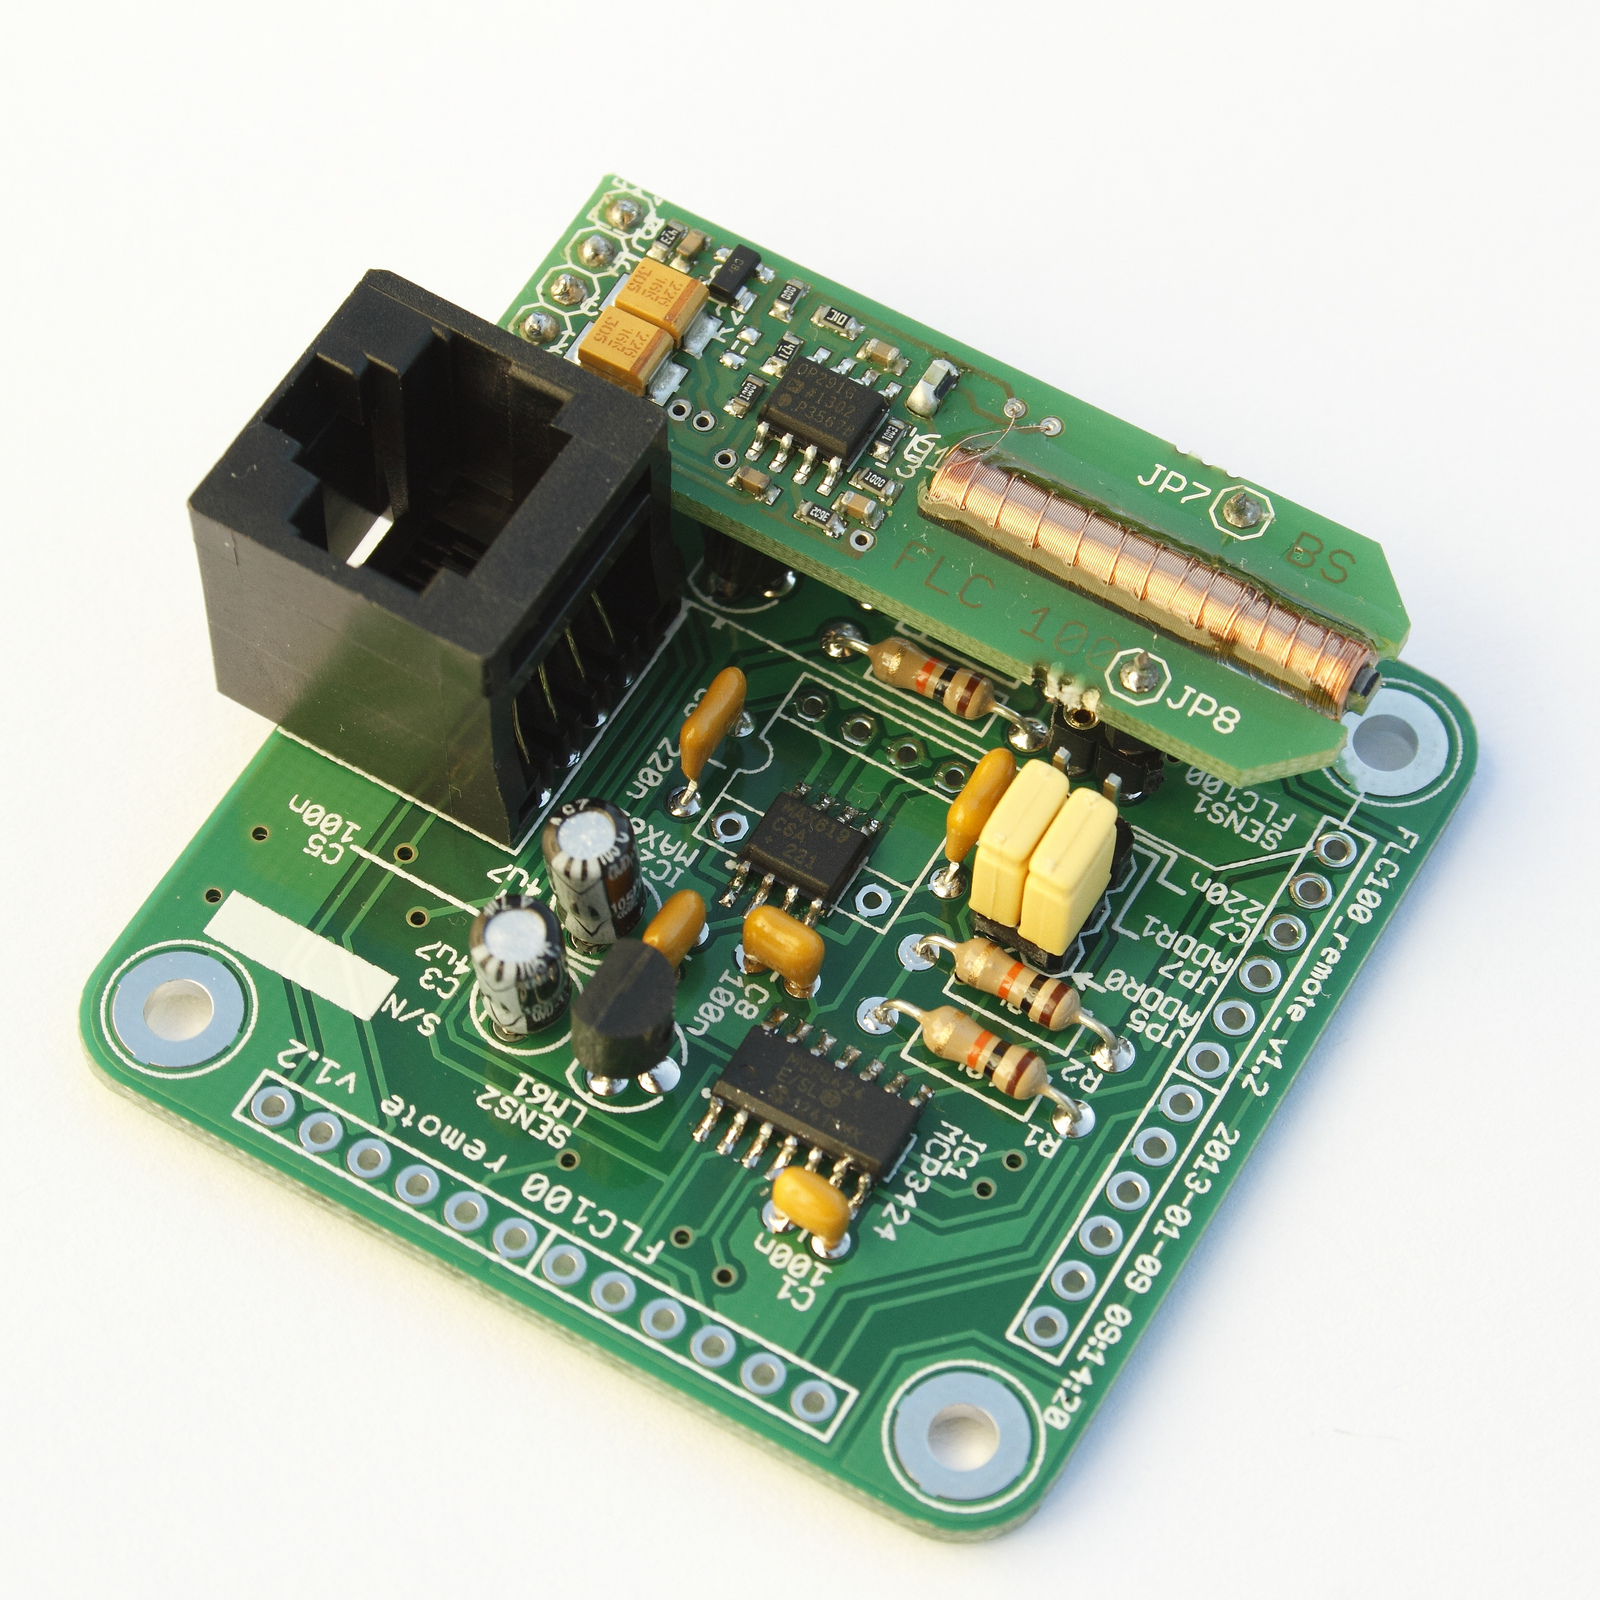
\includegraphics[keepaspectratio,width=\textwidth]{%
    images/flc100-sensor-pcb-v1-2}
  \caption[Completed sensor PCB (single-axis)]{%
    Completed sensor \pcb\ (single-axis). %
    \photoCredits{%
      \href{http://www.flickr.com/photos/stevemarple/10787290503/}{%
        \copyright Steve Marple. CC BY-SA 3.0.}}}
  \label{fig:sensor-pcb-v1.2}
\end{figure}
\begin{figure}
  \centering
  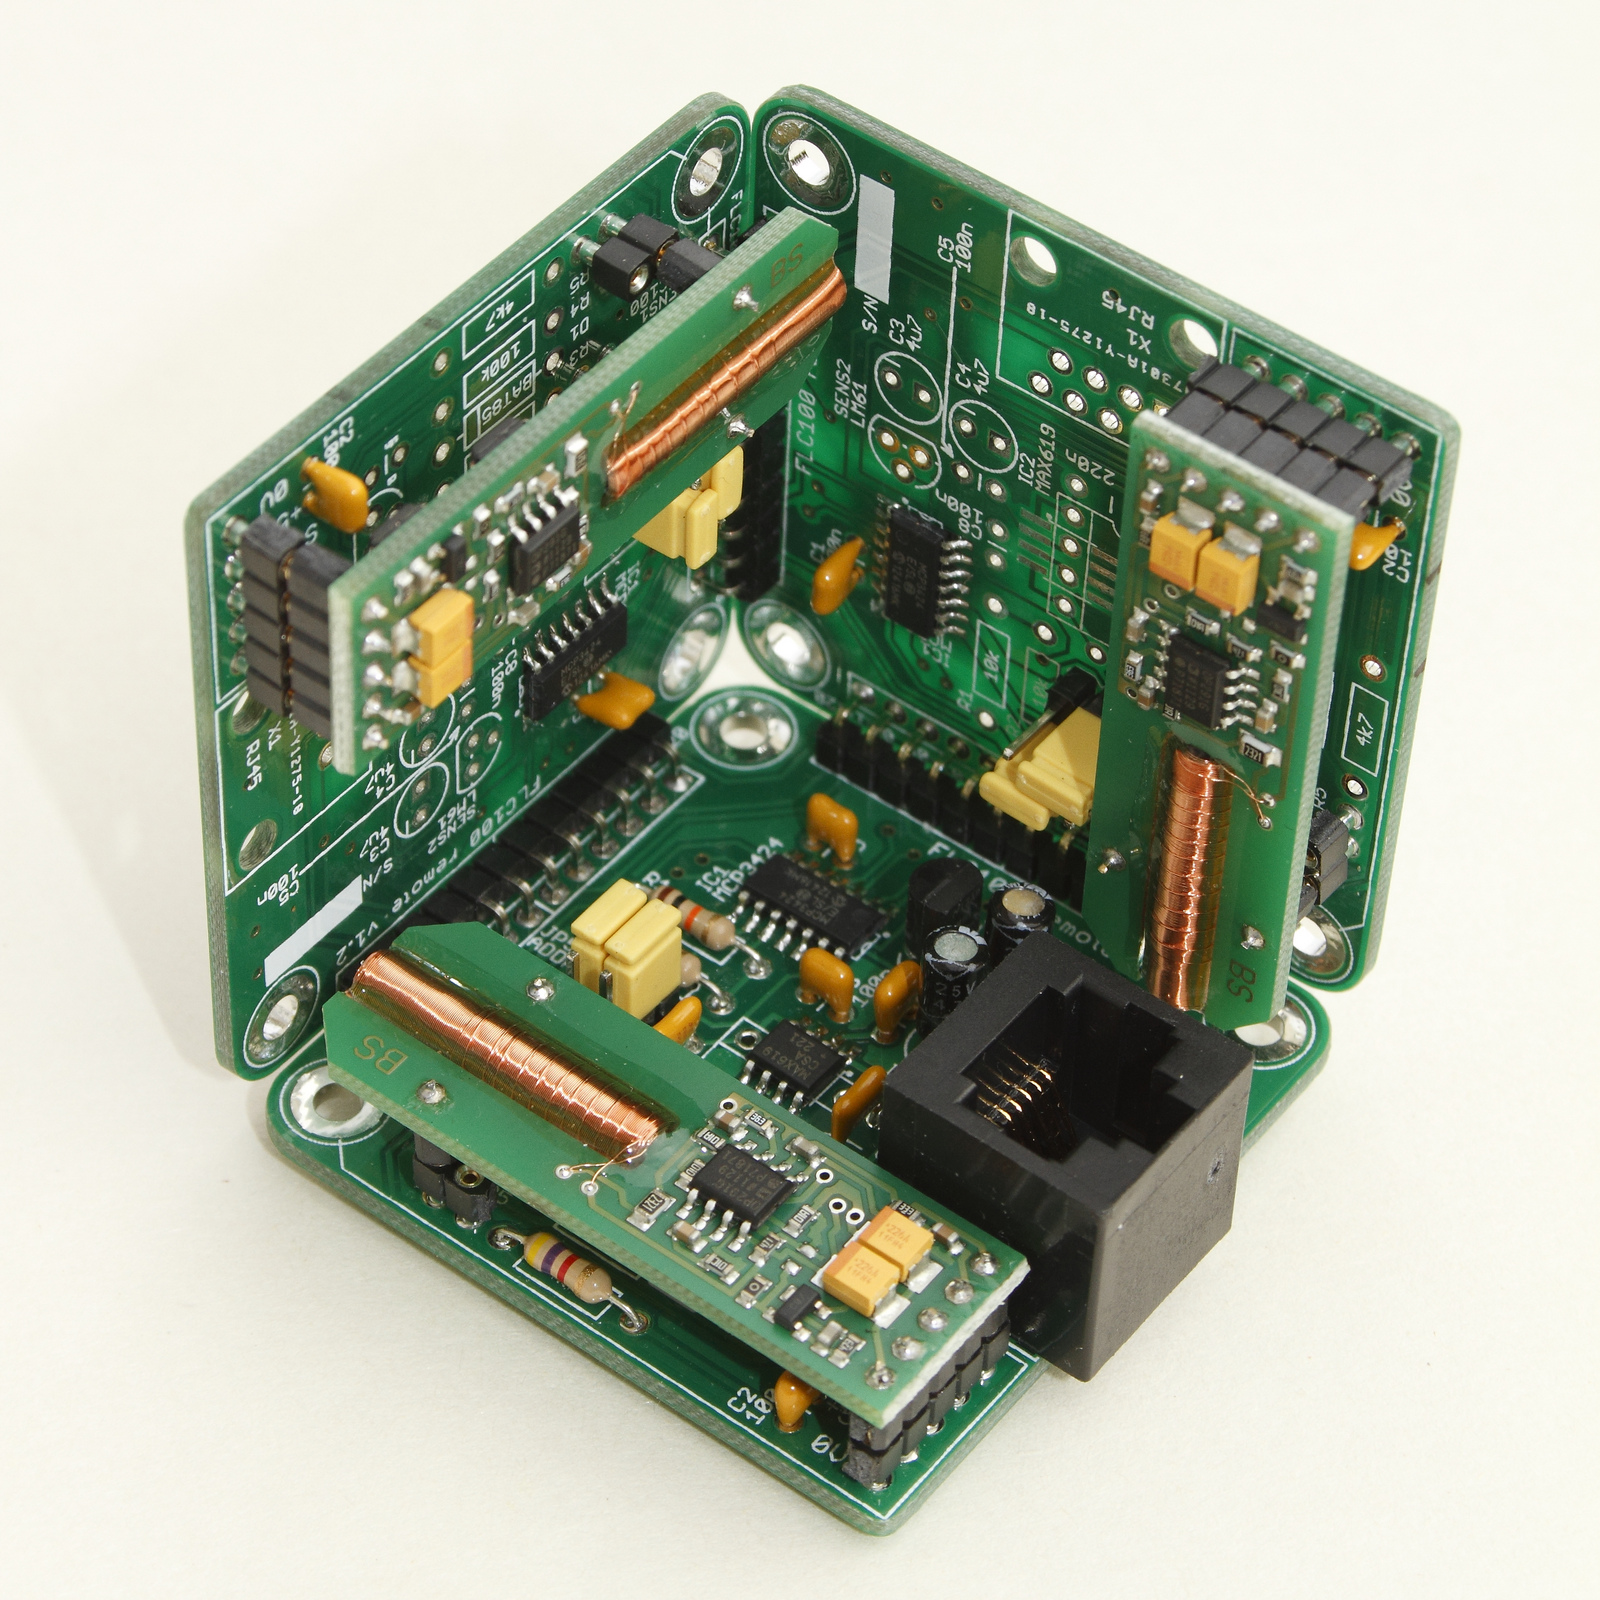
\includegraphics[keepaspectratio,width=\textwidth]{%
    images/flc100-sensor-pcb-v1-2-3d}
  \caption[Completed sensor PCB (three-axis)]{%
    Completed sensor \pcb\ (three-axis). %
    \photoCredits{%
      \href{http://www.flickr.com/photos/stevemarple/8521787269/}{%
        \copyright Steve Marple. CC BY-SA 3.0.}}}
  \label{fig:sensor-pcb-v1.2-3d}
\end{figure}

\subsection{Order of assembly}
Fit components in order:
\begin{buildorder}
\item Turned pin sockets for the FLC100 sensor. Accurate alignment is
  important so use a peice of solderless breadboard to hold the male
  turned-pin headers (\figurename~\ref{fig:flc100-step-1}). Insert the
  headers so that the conical part is pointing downwards. Fit the
  upside down turned-pin sockets onto the headers
  (\figurename~\ref{fig:flc100-step-2}). Place the \pcb\ onto the
  upside-down sockets (\figurename~\ref{fig:flc100-step-3}) and solder
  all 7 connections. Remove from the breadboard, leaving the male
  headers in place. Carefully position the FLC100 sensor onto the male
  turned-pin headers. The top-side of the FLC100 has two yellow
  capacitors and the letters BS the circuit board. Solder the FLC100
  sensor to the header. Gently remove the FLC100 sensor and place in
  an anti-static bag.
  \begin{figure}[p]
    \centering
    \todo[Take photo and insert]
    %%\includegraphics[width=10cm,keepaspectratio]{%
     %% images/flc100-step-1}
    \caption{Fit the male turned-pin headers.}
    \label{fig:flc100-step-1}
  \end{figure}
  \begin{figure}[p]
    \centering
    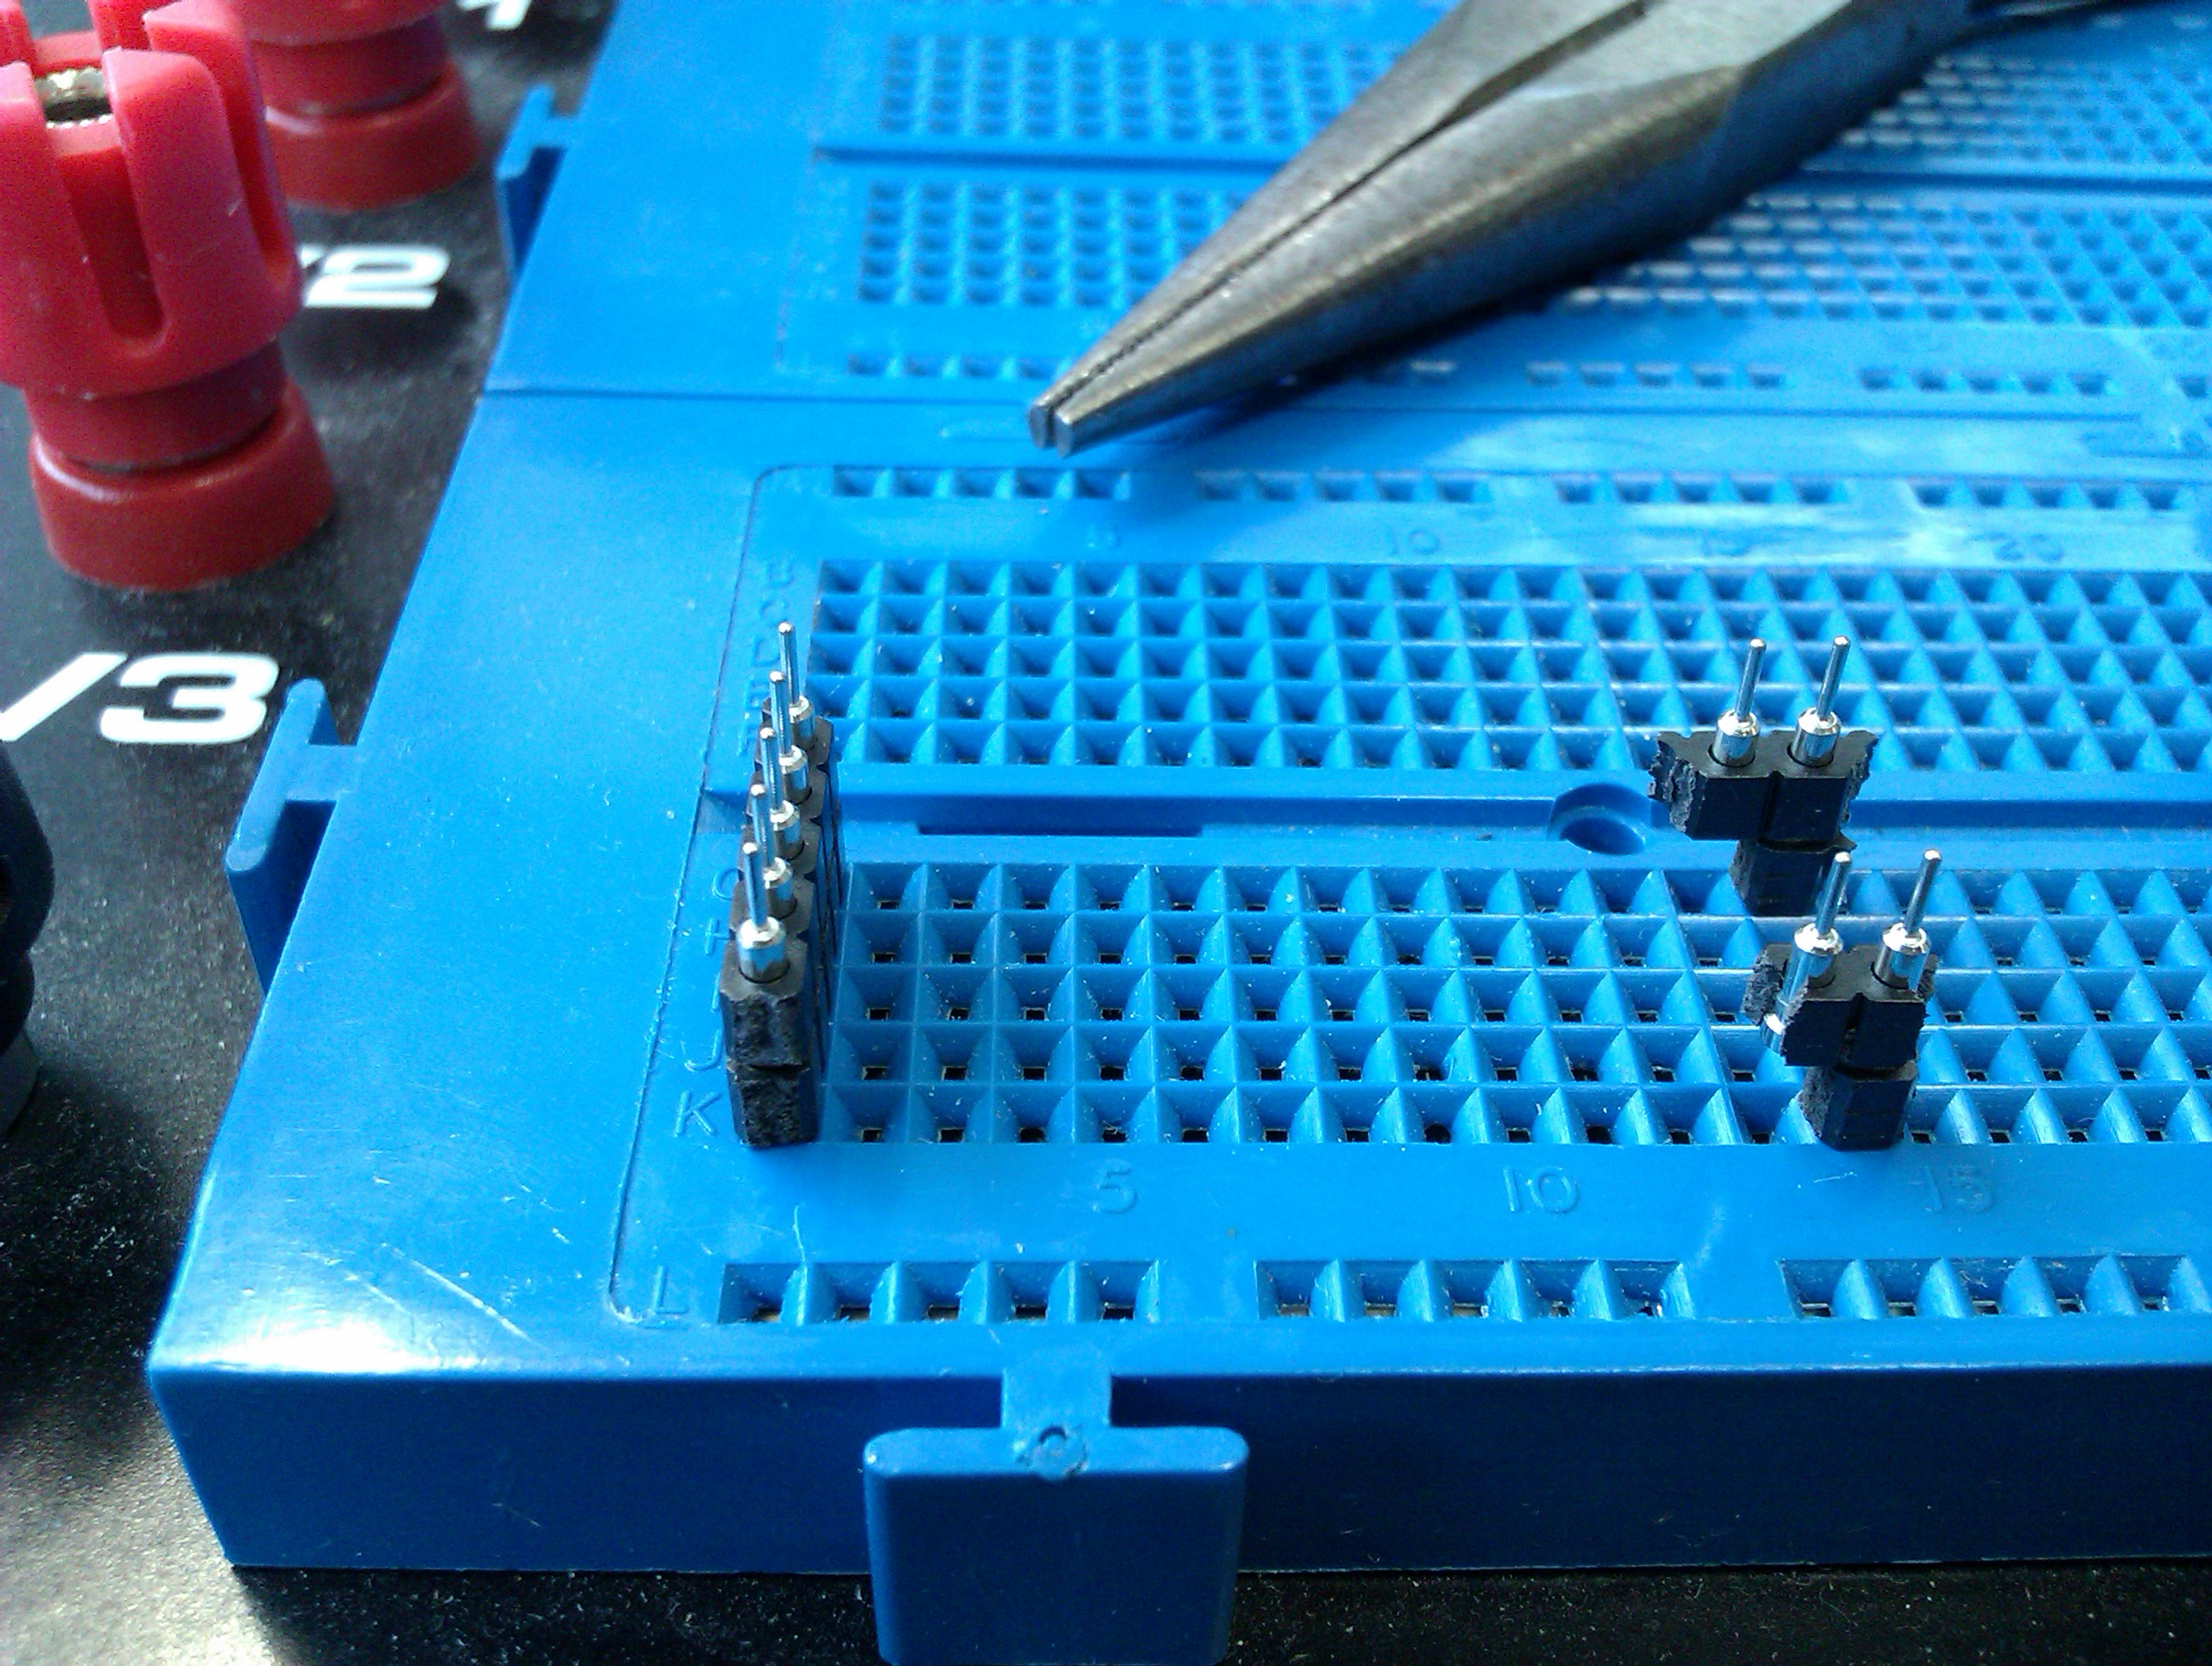
\includegraphics[width=10cm,keepaspectratio]{%
      images/flc100-step-2}
    \caption{Fit the female turned-pin sockets.}
    \label{fig:flc100-step-2}
  \end{figure}
  \begin{figure}[p]
    \centering
    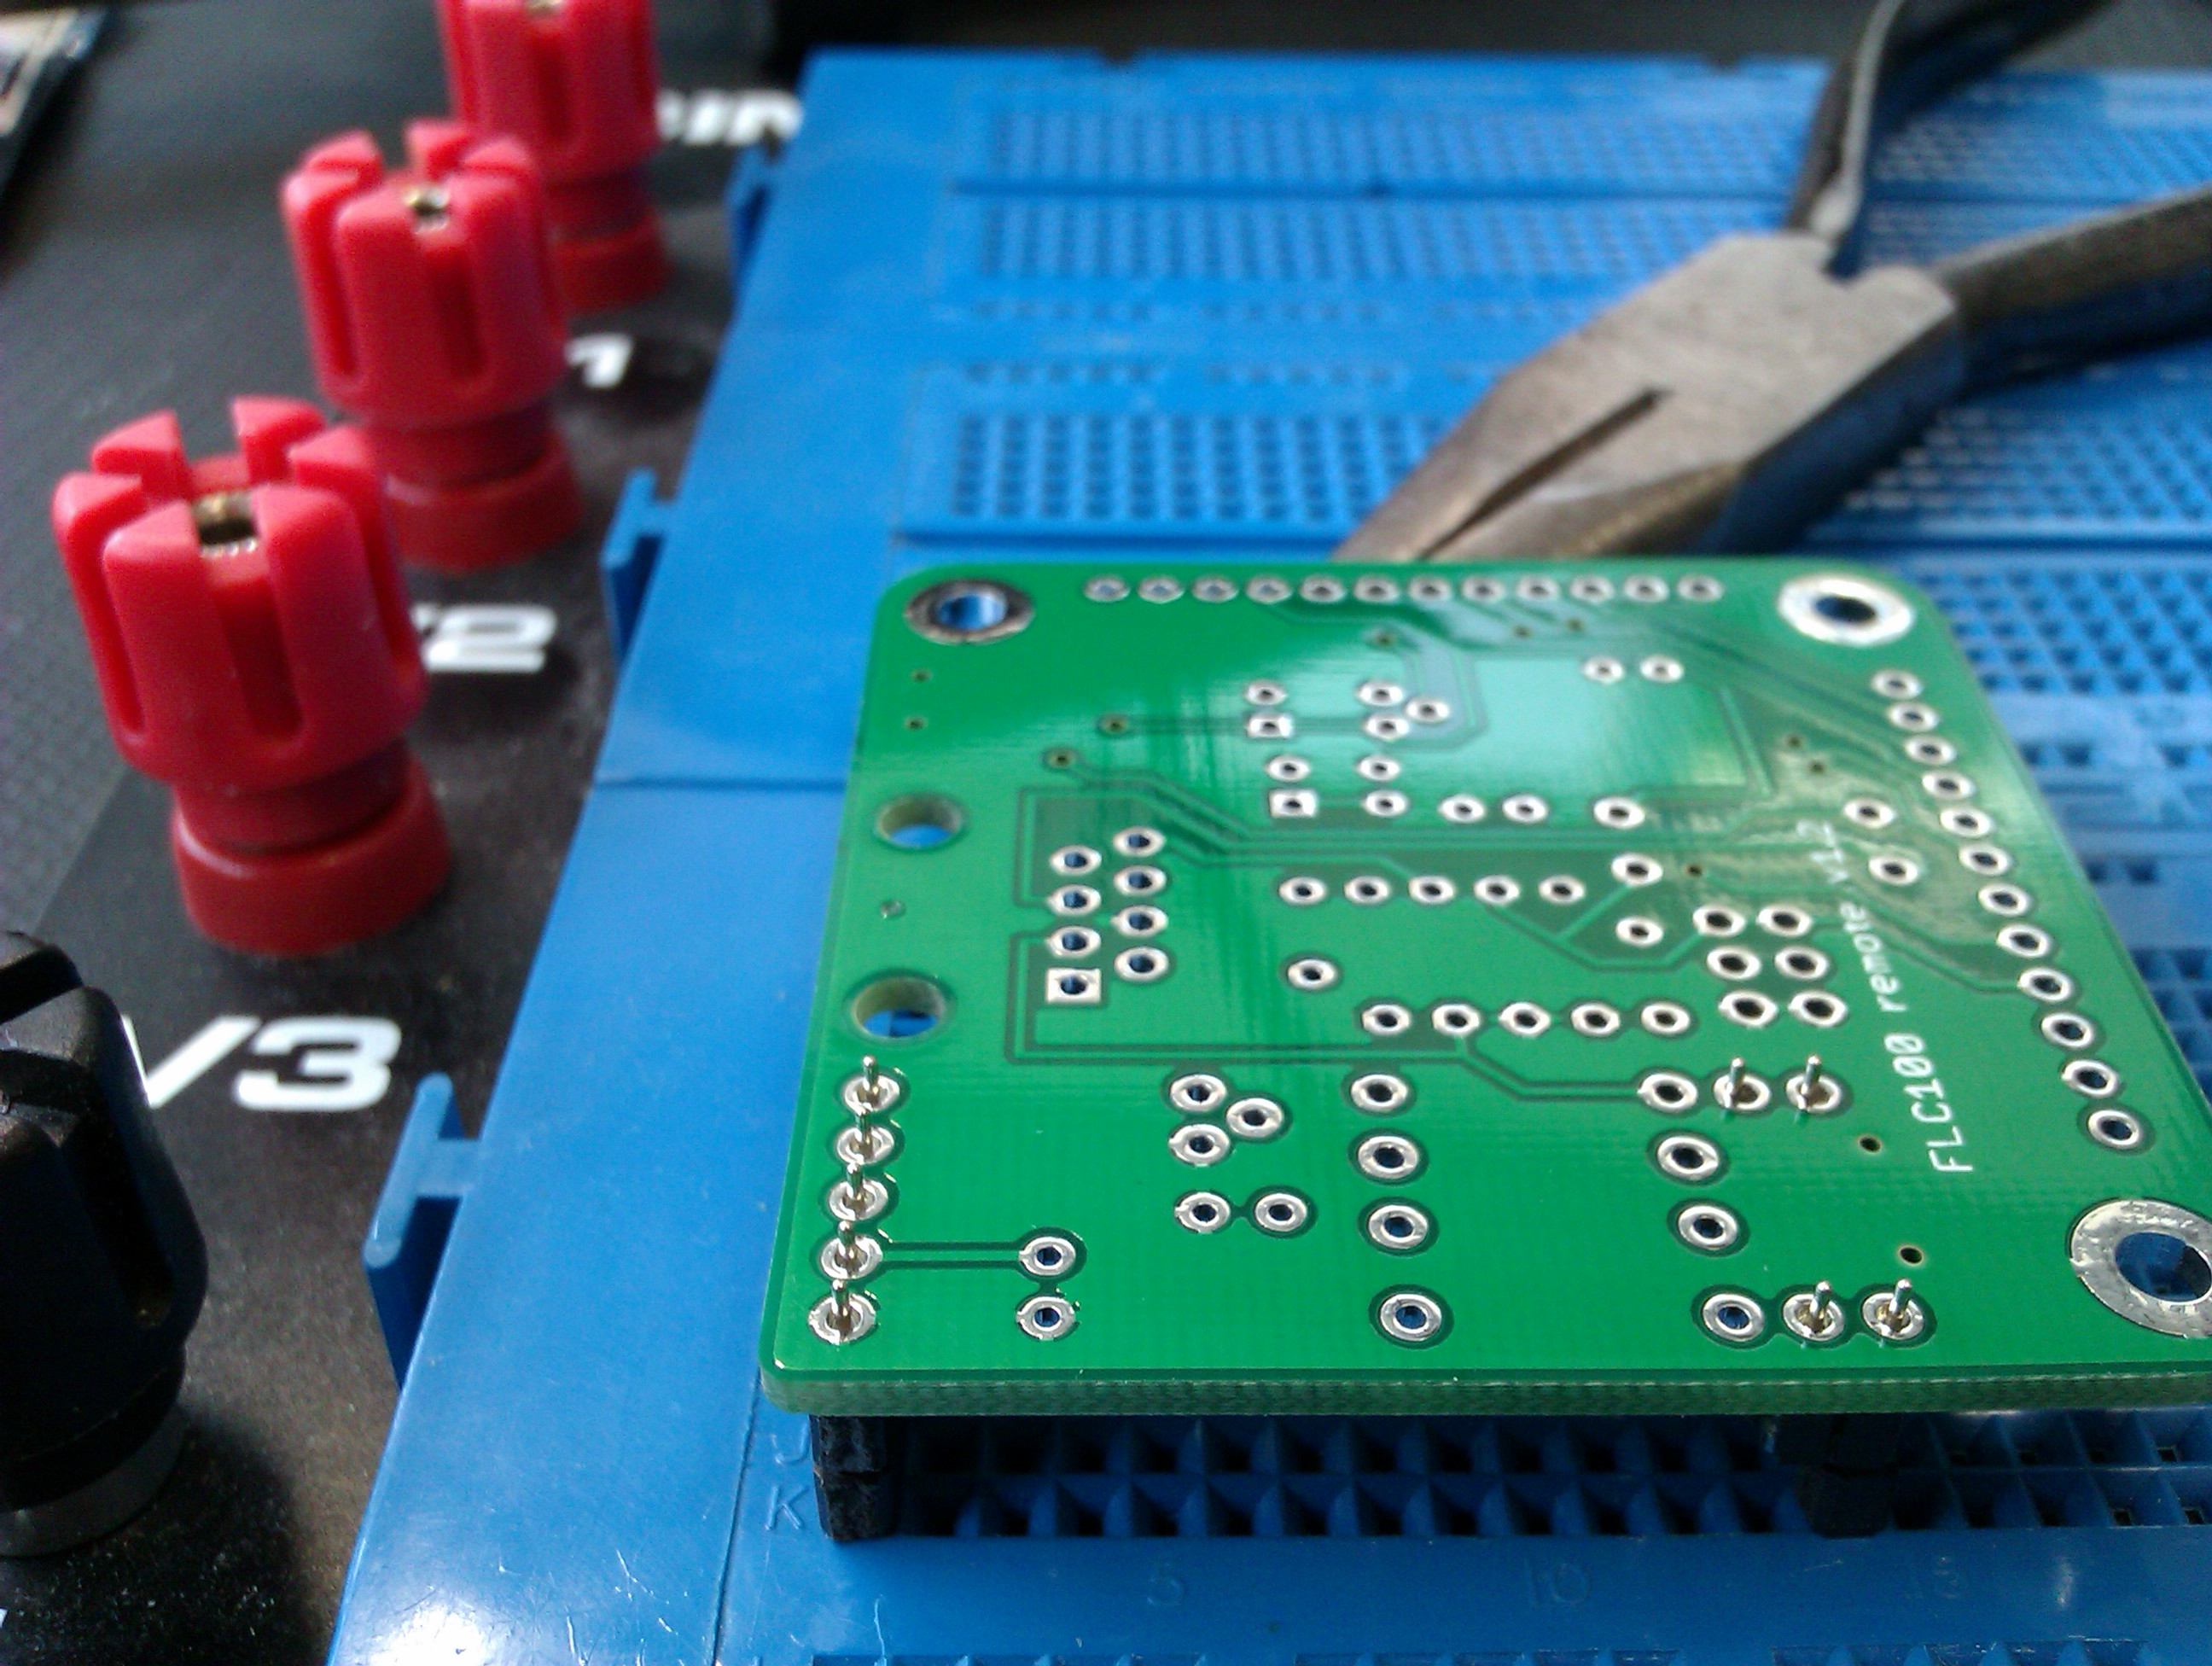
\includegraphics[width=10cm,keepaspectratio]{%
      images/flc100-step-3}
    \caption[Place the sensor PCB onto the female turned-pin
    sockets.]{%
      Place the sensor \pcb\ onto the female turned-pin sockets. The
      pliers are used to support the other side of the \pcb.}
    \label{fig:flc100-step-3}
  \end{figure}
\item IC1 (MAXMCP3424).
\item IC2 (MAX619).
\item R1, R2, R3 (\kohm{10}).
\item R4 (\kohm{100}).
\item R5 (\kohm{4.7}).
\item C1, C2, C5, C8 (\nF{100}).
\item C9 (\nF{10}).  
\item C6, C7 (\nF{220}).
\item C3, C4 (\uF{4.7}).
\item D1 (BAT85).
\item SENS2 (LM61).
\item JP5 and JP7 (fit as $2\times3$ male header).
\item X1 (RJ45 vertical jack).
\item Q1 (2N7000). This item is very sensitive to damage by
  electrostatic discharge!
\item SENS1. Gently fit the FLC100 sensor into the turned-pin
  sockets. Apply pressure only on the circuit boards, not the
  components or coil.
\end{buildorder}

\begin{landscape}
  % \thispagestyle{empty}
  \begin{figure}[p]
    \centering
    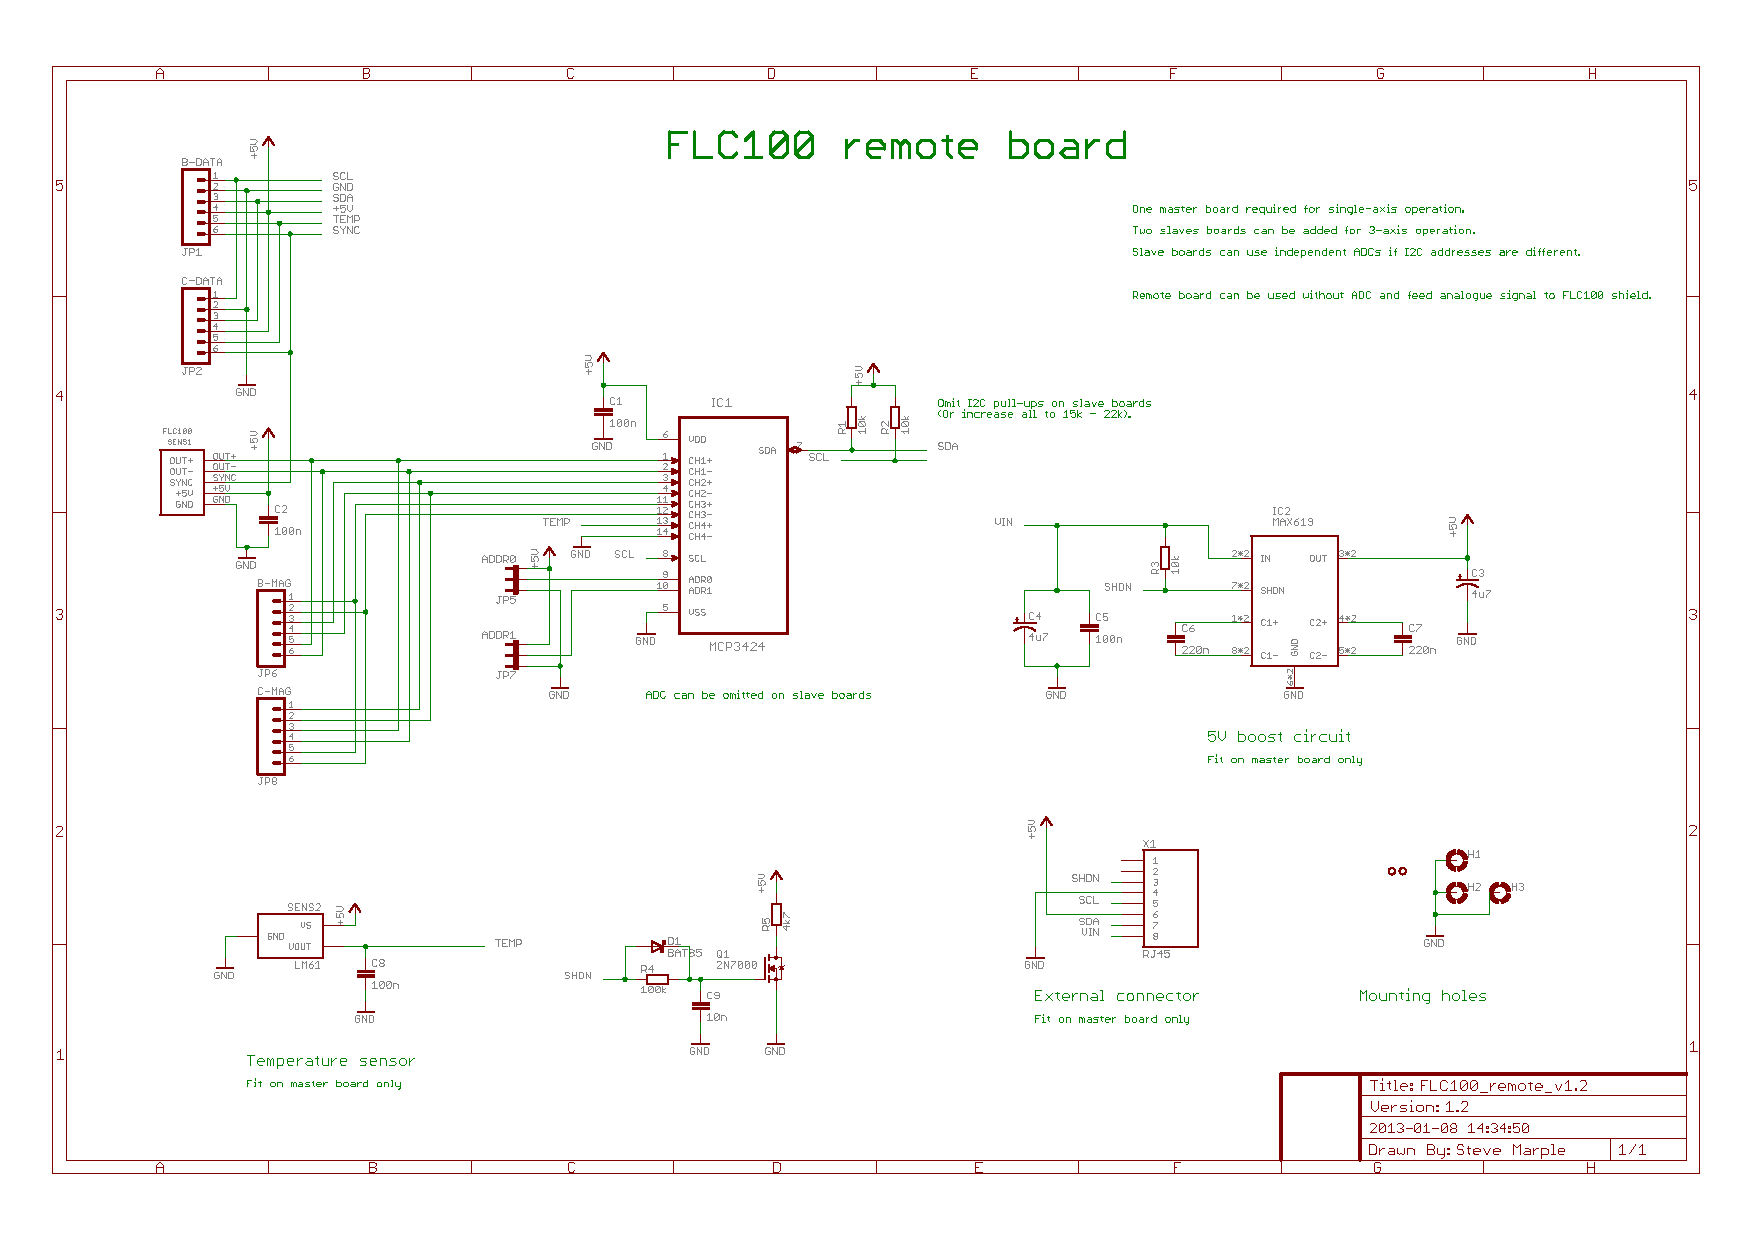
\includegraphics[keepaspectratio,width=28cm,height=16cm]{%
      {../../hardware/FLC100_shield/remote_v1.2/FLC100_remote_v1.2_sch}.pdf}
    \caption[Sensor PCB version 1.2 circuit diagram.]{%
      Sensor \pcb\ version 1.2 circuit diagram.}
    \label{fig:sensor-v1.2-pcb-cct-diag}
  \end{figure}
\end{landscape}
